\documentclass[12pt,letterpaper]{exam}
\usepackage[lmargin=1in,rmargin=1in,tmargin=1in,bmargin=1in]{geometry}
\usepackage{../style/exams}

% -------------------
% Course & Exam Information
% -------------------
\newcommand{\course}{MAT 104: Exam 2}
\newcommand{\term}{Spring -- 2023}
\newcommand{\examdate}{04/13/2023}
\newcommand{\timelimit}{85 Minutes}

\setbool{hideans}{true} % Student: True; Instructor: False

% -------------------
% Content
% -------------------
\begin{document}

\examtitle
\instructions{Write your name on the appropriate line on the exam cover sheet. This exam contains \numpages\ pages (including this cover page) and \numquestions\ questions. Check that you have every page of the exam. Answer the questions in the spaces provided on the question sheets. Be sure to answer every part of each question and show all your work.} 
\scores
%\bottomline
\newpage

% ---------
% Questions
% ---------
\begin{questions}

% Question 1
\newpage
\question[15] Complete the table of exact values for the trigonometric figures given below.
	{\def\arraystretch{3}
	\setlength{\tabcolsep}{2.5em}
	\begin{table}[!ht]
	\centering
	\begin{tabular}{|c||c|c|c|c|c|} \hline
	$\theta$ & $0$ & $\dfrac{\pi}{6}$ & $\dfrac{\pi}{4}$ & $\dfrac{\pi}{3}$ & $\dfrac{\pi}{2}$ \\ \hline \hline
	$\sin \theta$ &  &  &  &  &  \\ \hline
	$\cos \theta$ &  &  &  &  &  \\ \hline
	$\tan \theta$ &  &  &  &  &  \\ \hline
	\end{tabular}
	\end{table}
	}



% Question 2
\newpage
\question[15] Compute the exact values for the trigonometric functions given below.
	\begin{enumerate}[(a)]
	\item $\cos \!\left( \dfrac{5\pi}{6} \right)$
	\item $\tan \!\left( \dfrac{4\pi}{3} \right)$
	\item $\sin \!\left( -\dfrac{7\pi}{4} \right)$
	\item $\tan \!\left( \dfrac{3\pi}{2} \right)$
	\item $\sec \!\left( \dfrac{\pi}{4} \right)$
	\item $\cot \left( \pi \right)$
	\item $\csc \!\left( \dfrac{2\pi}{3} \right)$
	\end{enumerate}



% Question 3
\newpage
\question[10] Compute the exact values (in radians) for the inverse trigonometric functions given below.
	\begin{enumerate}[(a)]
	\item $\sin^{-1} \!\!\left( -\dfrac{1}{2} \right)$
	\item $\arccos \!\left( \dfrac{1}{2} \right)$
	\item $\tan^{-1} \!\left( -\sqrt{3} \right)$
	\item $\arcsin \!\left( \sin \left( \dfrac{7\pi}{6} \right) \right)$
	\item $\arctan(\infty)$
	\end{enumerate}
	


% Question 4
\newpage
\question[10] Given the right triangle below, compute the exact values of the indicated trigonometric functions. \pspace
\begin{minipage}{0.3\textwidth}
        \begin{enumerate}[(a)]
        \item $\sin \theta$
        \item $\cos \phi$
        \item $\tan \theta$
        \item $\sec \theta$
        \item $\csc \phi$
        \end{enumerate}
\end{minipage} \begin{minipage}{0.27\textwidth}        
	\[
	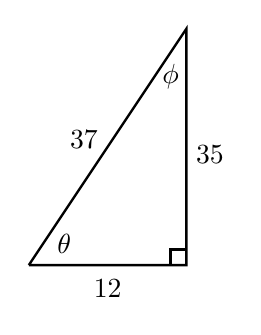
\begin{tikzpicture}
	\draw[line width=0.03cm] (0,0) -- (2,0) -- (2,3) -- (0,0);
	\draw[line width=0.03cm] (1.8,0) -- (1.8,0.2) -- (2,0.2);
	\node at (0.45,0.27) {$\theta$};
	\node at (1.8,2.4) {$\phi$};
	\node at (1,-0.3) {$12$};
	\node at (2.3,1.4) {$35$};
	\node at (0.7,1.6) {$37$};
	\end{tikzpicture}
	\]
\end{minipage}



% Question 5
\newpage
\question[10] Showing all your work, compute the expressions given below.
	\begin{enumerate}[(a)]
	\item $\sin(2\theta)$, if $\tan(\theta)= \dfrac{4}{3}$ and $0 < \theta < \dfrac{\pi}{2}$
	\item $\tan \!\left( \cos^{-1} \left( -\dfrac{3}{4} \right) \right)$
	\end{enumerate}



% Question 6
\newpage
\question[10] Complete the parts given below.
	\begin{enumerate}[(a)]
	\item Find the value of $\sin^2(1 - x) + \cos^2(1 - x)$.
	\item Express $\sin(\theta \pm \phi)$ in terms of $\sin \theta$, $\sin \phi$, $\cos \theta$, and $\cos \phi$. 
	\item Express $\cos(2\theta)$ in terms of $\cos \theta$ and $\sin \theta$. 
	\item Express $\sin^2 \theta$ in terms of $\cos(2\theta)$.
	\item Express $\cos^2 \theta$ in terms of $\cos(2\theta)$. 
	\end{enumerate}



% Question 7
\newpage
\question[10] Given that $\dfrac{11\pi}{12}= \dfrac{5\pi}{4} - \dfrac{\pi}{3}$, compute the exact value of $\cos \left( \dfrac{11\pi}{12} \right)$. 



% Question 8
\newpage
\question[10] Compute the exact area of the triangle shown below. 
	\[
	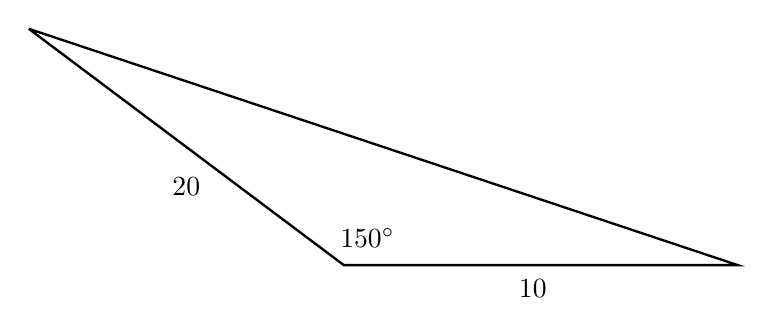
\begin{tikzpicture}
	\draw[line width=0.03cm] (-4,3) -- (0,0) -- (5,0) -- (-4,3);
	\node at (0.3,0.35) {$150^\circ$};
	\node at (2.4,-0.3) {$10$};
	\node at (-2,1) {$20$};
	\end{tikzpicture}
	\]



% Question 9
\newpage
\question[10] Compute the exact area of the triangle shown below.
	\[
	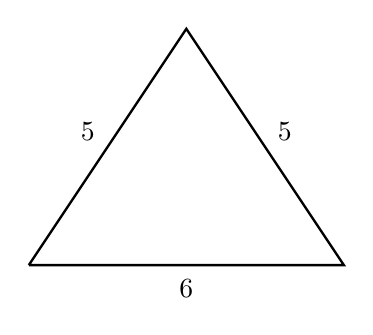
\begin{tikzpicture}
	\draw[line width=0.03cm] (-2,0) -- (0,3) -- (2,0) -- (-2,0);
	\node at (-1.25,1.7) {$5$};
	\node at (1.25,1.7) {$5$};
	\node at (0,-0.3) {$6$};
	\end{tikzpicture}
	\]



% Question 10
\newpage
\question[10] Find the exact value of the side $s$ in the triangle below. 
	\[
	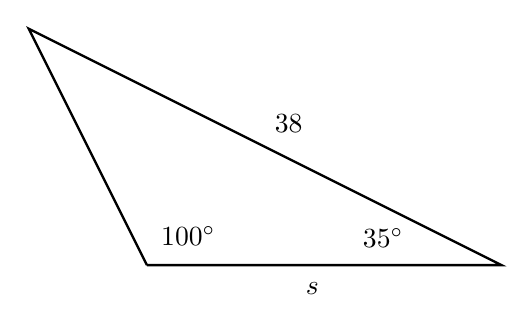
\begin{tikzpicture}[scale=1.5]
	\draw[line width=0.03cm] (-1,0) -- (-2,2) -- (2,0) -- (-1,0);
	\node at (-0.65,0.25) {$100^\circ$};
	\node at (1.0,0.23) {$35^\circ$};
	\node at (0.2,1.2) {$38$};
	\node at (0.4,-0.2) {$s$};
	\end{tikzpicture}
	\]



% Question 11
\newpage
\question[10] Find the exact value of the side $s$ in the triangle below.
	\[
	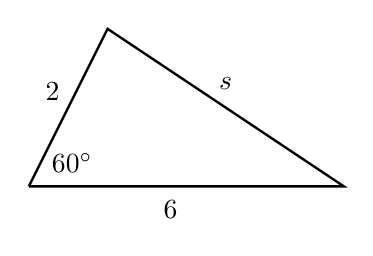
\begin{tikzpicture}
	\draw[line width=0.03cm] (0,0) -- (1,2) -- (4,0) -- (0,0);
	\node at (0.55,0.3) {$60^\circ$};
	\node at (0.3,1.2) {$2$};
	\node at (1.8,-0.3) {$6$};
	\node at (2.5,1.3) {$s$};
	\end{tikzpicture}
	\]



% Question 12
\newpage
\question[10] Verify the trigonometric identity given below.
	\[
	\dfrac{\tan \theta - \cot \theta}{\sin \theta \cos \theta}= \sec^2 \theta - \csc^2 \theta
	\]



% Question 13
\newpage
\question[10] Verify the trigonometric identity given below.
	\[
	\dfrac{\sin x}{1 + \cos x} + \dfrac{\cos x - 1}{\sin x}= 0 
	\]



% Question 14
\newpage
\question[10] Find all the solutions to the equation below.
	\[
	3\sin \theta= \sqrt{3} \cos \theta
	\]



% Question 15
\newpage
\question[10] Find all the solutions to the equation below.
	\[
	2 \cos(2x) \sin x + \cos(2x)= 0 
	\]


\end{questions}
\end{document}